
\ifnum \Version=1
\question[6]  An object is moving along a path given by $\mathbf r(t)$ for $t \ge 0$, where $ \mathbf r '(t) = \mathbf v = \langle 4, t, 2\sqrt{2t\,} \rangle$. Please show your work for the parts below. You can use your results for each part using results from previous parts of this question.   

\begin{parts}
    \part Determine the speed, acceleration vector, and unit tangent vector for the curve. 
    \ifnum \Solutions=1 {\color{DarkBlue} 
        \begin{align}
          s = \left | \mathbf v \right| &= \sqrt{4^2 + t^2  +(2\sqrt{2t})^2} = \sqrt{t^2 + 8t + 16} = \sqrt{(t+4)^2} = t + 4\\
          \frac{d}{dt} 2\sqrt{2t\,} &= 2\left( \frac{d}{dt} \sqrt{2t\,} \right) =2 \cdot \frac12 \left( 2t\right)^{-1/2}\frac{d}{dt}(2t) = \frac{2}{\sqrt{2t\,}} \\
          \mathbf a &= \mathbf v ' (t) = \langle 0,1, \frac{2}{\sqrt{2t\,}} \rangle = \mathbf j + \frac{2}{\sqrt{2t\,}}\mathbf k\\
          \mathbf T &= \frac{\mathbf v}{s} 
          = \frac{1}{t+4} \langle 4, t, 2\sqrt{2t\,} \rangle  
          = \frac{4}{t+4}\mathbf i + \frac{t}{t+4}\mathbf j + \frac{2\sqrt{2t\,}}{t+4}\mathbf k
        \end{align}
        } 
    \else
      \vspace{6cm}
    \fi
    \part Determine the length of the curve, $L$, from the point where $t=4$ to $t=8$. Simplify your answer as much as possible. 
    \ifnum \Solutions=1 {\color{DarkBlue} \\[12pt]
        Apply the arc length formula.
        \begin{align}
            L &= \int_4^8 |\mathbf v| \, dt = \int_4^{8} t+4 \, dt = \left. \left(\frac{t^2}{2} +4t\right)\right|_4^{8} = (32+32) - (8+16) = 64 - 24 = 40
        \end{align}
        The question asked to simplify your work as much as possible, so for full credit you would not want to leave your answer as something like $64-24$. 
        } 
    \else
      \vspace{4cm}
    \fi         
    \part Suppose the object starts at the origin, so that $\mathbf r(0) = \mathbf 0$. Determine the value of $t$ that corresponds to the point on the curve that is a distance of 10 units away from the origin along the curve. In other words, determine the value of $t$ so that the arc length between the origin and $\mathbf r(t)$ is 10. 
    \ifnum \Solutions=1 {\color{DarkBlue} \\[12pt]
        We can use the arc length parameter
        $\displaystyle s(t) = \int_{t_0}^t |\mathbf v| \, d\tau$, with $s=10$, $t_0 = 0$, and solve for $t$. 
        \begin{align}
            s(t) = \int_{t_0}^t |\mathbf v| \, d\tau = 
            10 &=  \int_{0}^t \tau+4 \, d\tau \\
            10 &= \left. \left(\frac{\tau^2}{2} +4\tau\right)\right|_0^{t} \\
            10 &= \frac{t^2}{2} +4t \\
            0 &= t^2 + 8t - 20 \\
            0 &= (t+10)(t-2)
        \end{align}
        We should ignore $t=-10$ because we were given that $t\ge0$. So the value of $t$ is $t=2$. 
        } 
    \else
      \vspace{7cm}
    \fi 
    
\end{parts}
\fi





\ifnum \Version=2
\question[6]  An object is moving along a path given by $\mathbf r(t) = \langle t , \cos t, \sin t \rangle$ for $t \in \mathbb R$. Please show your work for the parts below. You can use your results for each part using results from previous parts of this question.   

\begin{parts}
    \part Determine the velocity, acceleration, and unit tangent vectors for the curve. 
    \ifnum \Solutions=1 {\color{DarkBlue} 
        \begin{align}
          \mathbf v &= \mathbf r '(t) = \mathbf i - \sin t\mathbf j + \cos t \mathbf k \\
          |\mathbf v | &= \sqrt 2 \\
          \mathbf T &= \frac{1}{\sqrt{2}} \langle1,-\sin t, \cos t\rangle \\ 
          \mathbf a &= \mathbf v ' (t) = \langle 0,-\cos t, -\sin t \rangle 
        \end{align}
        } 
    \else
      \vspace{6cm}
    \fi
    \part Determine the length of the curve, $L$, from the point where $t=4$ to $t=12$. 
    \ifnum \Solutions=1 {\color{DarkBlue} \\[12pt]
        Apply the arc length formula.
        \begin{align}
            |\mathbf v | &= \sqrt 2 \\
            L &= \int_1^4 |\mathbf v| \, dt = \int_4^{12} \sqrt 2 \, dt = \sqrt 2 \, t|_4^{12} = \sqrt2(12 - 4) = 8\sqrt 2
        \end{align}
        For full credit do not leave your answer as $\sqrt 2 \, t|_4^{12}$. 
        } 
    \else
      \vspace{4cm}
    \fi         
    \part Determine the curvature of $\mathbf{r}(t)$ when $t=0$. 
    \ifnum \Solutions=1 {\color{DarkBlue} \\[12pt]
        There are a few different formulas for curvature. Let's use the formula
            \begin{align}
                \kappa = \frac{1}{|\mathbf v | } \left| \frac{d\mathbf T}{dt} \right| 
            \end{align}
            Then
            \begin{align}
                |\mathbf v | &= \sqrt 2 \\
                \frac{d\mathbf T}{dt} &= \frac{1}{\sqrt 2}\langle 0, -\cos t, -\sin t\rangle \\
                \left| \frac{d\mathbf T}{dt} \right| &= \frac{1}{\sqrt 2} \\
                \kappa &= \frac{1}{|\mathbf v | } \left| \frac{d\mathbf T}{dt} \right| = \frac{1}{\sqrt 2} \, \frac{1}{\sqrt 2} = \frac12
            \end{align}
        Note that there are formulas for curvature that are in sections of the textbook that we didn't cover. You aren't expected to know them for your exam, but if you like you can use them. One such formula is $\displaystyle \kappa = \frac{|\mathbf v \times \mathbf a|}{ |\mathbf v|^3 }$: 
        \begin{align}
            \mathbf v \times \mathbf a &= \begin{vmatrix} \mathbf i & \mathbf j & \mathbf k \\ 1&-\sin t&\cos t \\ 0&-\cos t&-\sin t
            \end{vmatrix} = \langle 1, \sin t, -\cos t \rangle \\
            |\mathbf v \times \mathbf a| &= \sqrt 2 \\ 
            \kappa &= \frac{|\mathbf v \times \mathbf a|}{ |\mathbf v|^3 }= \frac{\sqrt 2}{(\sqrt 2)^3} = \frac12
        \end{align}
        The curvature is $\frac12$ for all $t$. 
        } 
    \else
      \vspace{7cm}
    \fi 
    
\end{parts}
\fi








\ifnum \Version=3

\question[6]  An object is moving in the $xy$-plane along a path given by $\mathbf r(t) = \langle t , t^2+1 \rangle$ for $t \in \mathbb R$. Please show your work for the parts below. You can use your results for each part using results from previous parts of this question.   

    \begin{parts}
        \part Determine the velocity, acceleration vector, and unit tangent vector for the curve. 
        \ifnum \Solutions=1 {\color{DarkBlue} 
            \begin{align}
              \mathbf v &= \mathbf r '(t) = \mathbf i + 2t\mathbf j \\
              \mathbf a &= \mathbf v ' (t) = 2\mathbf j \\
              \mathbf T &= \frac{\mathbf v}{|\mathbf v |} = \frac{1}{\sqrt{4t^2+1}}\left( \mathbf i + 2t\mathbf j \right)
            \end{align}
            } 
        \else
          \vspace{5cm}
        \fi
        \part Determine the curvature of $\mathbf{r}(t)$ when $t=0$. 
        \ifnum \Solutions=1 {\color{DarkBlue} \\[12pt]
            A planar curve of the form $y = f(x)$ can be parameterized using $\mathbf r(x) = x\mathbf i + f(x)\mathbf j$, and in such a case it can be shown that we can compute the curvature using
            $$\kappa = \frac{|f''(x)|}{\left[ 1+ (f'(x))^2\right]^{3/2}}$$
            For this problem, we can parameterize the curve by setting $x = t$ and $f = f(y) = f(x(t)) = t^2+1$, and use this curvature formula as follows.  
            \begin{align}
                \kappa(t) &= \frac{|f''(t)|}{ ( 1+(f'(t))^2 )^{3/2}} = \frac{2}{(1+(2t)^2)^{3/2}} \\
                \kappa(0) &= \frac{2}{(1+0)^{3/2}} = \frac{2}{1^{3/2}} = 2
            \end{align}
            Note that it is also possible to calculate curvature in other ways, as there are other formulas for curvature. 
            } 
        \else
          \vspace{7cm}
        \fi 
    
    
        \part Given that the principal normal vector when $t=0$ is $\mathbf N=\mathbf j$, determine the equation of the osculating circle when $t=0$.
        \ifnum \Solutions=1 {\color{DarkBlue} \\[12pt]
            The circle has radius $1/\kappa = \frac12$ and touches the curve at the point where $t=0$. This corresponds to the point $(0,1)$, because $\mathbf r(t) = \langle t , t^2+1 \rangle$, and 
            \begin{align}
                \mathbf r(0) = \langle 0, 1 \rangle
            \end{align}
            The normal vector points in the direction of $\mathbf j$, so the circle has center that is $\frac12$ units above the point $(0,1)$, which is the point $(0,1+\frac12)$. The circle has the equation 
            $$(x-0)^2+\left(y - \frac32\right)^2 = \left( \frac12 \right)^2$$
            We could also write this as
            $$x^2+\left(y - \frac32\right)^2 =  \frac14 $$    
            Sketching wasn't necessary but if we put the curve and the circle into Desmos, the picture below is what we get. Note that the circle touches the curve at the point $(0,1)$, that it lies above the curve, and has radius $1/2$. 

            \begin{center}
            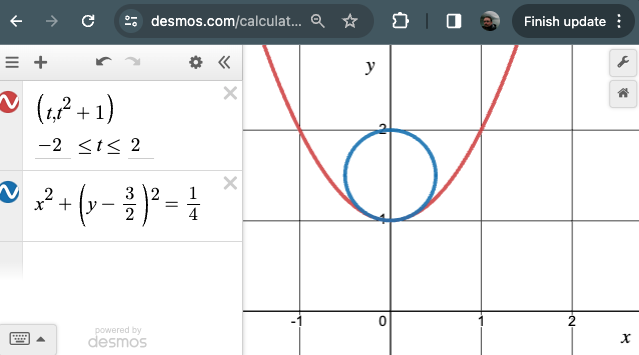
\includegraphics[width=0.75\paperwidth]{202402/Exam1/Images/OscCircle01.png}                            
            \end{center}
            } 
        \else
          \vspace{4cm}
        \fi  
    
        
    \end{parts}
\fi




\ifnum \Version=4
\question[6]  An object is moving in the $xy$-plane along a path given by $\mathbf r(t) = \langle t , ((t-4)^2+1)\rangle = \langle t, t^2 - 8t +17\rangle$ for $t \ge 0$. Please show your work for the parts below. You can use your results for each part using results from previous parts of this question.   

\begin{parts}
    \part Determine the velocity and acceleration vectors for the curve for any $t\ge 0$. 
    \ifnum \Solutions=1 {\color{DarkBlue} 
        \begin{align}
          \mathbf v &= \mathbf r '(t) = \mathbf i + (2t-8)\mathbf j \\
          \mathbf a &= \mathbf v ' (t) = 2\mathbf j 
        \end{align}
        } 
    \else
      \vspace{2cm}
    \fi
    \part Determine the curvature of $\mathbf{r}(t)$ when $t=4$. 
    \ifnum \Solutions=1 {\color{DarkBlue} \\[12pt]
        Setting $x = t$ and $f(x) = x^2-8x+17$ we may calculate the curvature using the formula 
        \begin{align}
            \kappa &= \frac{|f''(x)|}{ ( 1+(f'(x))^2 )^{3/2}} = \frac{2}{(1+(2x-8)^2)^{3/2}} \\
            \kappa(4) &= \frac{2}{(1+(2(4)-8)^2)^{3/2}} = \frac{2}{1^{3/2}} = 2
        \end{align}
        The above formula was introduced in one of the homework problems for Section 13.4. Note that it is also possible to calculate curvature in other ways, as there are several other formulas for curvature. 
        } 
    \else
      \vspace{7cm}
    \fi 

    \part Determine the unit tangent vector $\mathbf T$ when $t=4$. 
    \ifnum \Solutions=1 {\color{DarkBlue} \\[12pt]
        Using the formulas for these vectors we obtain
        \begin{align}
        | \mathbf v | &= \sqrt{1+(2t-8)^2} \\          
          \mathbf T &= \frac{\mathbf v}{|\mathbf v |} = \frac{\langle 1, 2t-8 \rangle}{\sqrt{1+(2t-8)^2}} \\
          \mathbf T(4) &= \langle 1,0\rangle
        \end{align}
        } 
    \else
      \vspace{5cm}
    \fi  

    \part Given that the principal normal vector when $t=4$ is $\mathbf N=\mathbf j$, determine the equation of the osculating circle when $t=4$.
    \ifnum \Solutions=1 {\color{DarkBlue} \\[12pt]
        The circle has radius $1/\kappa = \frac12$ and touches the curve at the point
        \begin{align}
            \mathbf r(4) = \langle 4, 1 \rangle
        \end{align}
        The normal vector points in the direction of $\mathbf j$, so the circle has center $(4,1+\frac12)$. The circle has the equation $(x-4)^2+(y-3/2)^2 = 1/4$. 
        } 
    \else
      \vspace{4cm}
    \fi  

    
\end{parts}
\fi









\ifnum \Version=5
\question[6]  An object is moving along a path given by $\mathbf r(t) = \langle t , \cos t, \sin t \rangle$ for $t \in \mathbb R$. Please show your work for the parts below. You can use your results for each part using results from previous parts of this question.   

\begin{parts}
    \part Determine the velocity, acceleration, and unit tangent vectors for the curve. 
    \ifnum \Solutions=1 {\color{DarkBlue} 
        \begin{align}
          \mathbf v &= \mathbf r '(t) = \mathbf i - \sin t\mathbf j + \cos t \mathbf k \\
          |\mathbf v | &= \sqrt 2 \\
          \mathbf T &= \frac{1}{\sqrt{2}} \langle1,-\sin t, \cos t\rangle \\ 
          \mathbf a &= \mathbf v ' (t) = \langle 0,-\cos t, -\sin t \rangle 
        \end{align}
        } 
    \else
      \vspace{6cm}
    \fi
    \part Determine the length of the curve, $L$, from the point where $t=1$ to $t=4$. 
    \ifnum \Solutions=1 {\color{DarkBlue} \\[12pt]
        Apply the arc length formula.
        \begin{align}
            |\mathbf v | &= \sqrt 2 \\
            L &= \int_1^4 |\mathbf v| \, dt = \int_1^4 \sqrt 2 \, dt = \sqrt 2 \, t|_1^4 = \sqrt2(4-1) = 3\sqrt 2
        \end{align}
        For full credit do not leave your answer as $\sqrt 2 \, t|_1^4$. 
        } 
    \else
      \vspace{4cm}
    \fi         
    \part Determine the curvature of $\mathbf{r}(t)$ when $t=0$. 
    \ifnum \Solutions=1 {\color{DarkBlue} \\[12pt]
        There are a few different formulas for curvature. Let's use the formula
            \begin{align}
                \kappa = \frac{1}{|\mathbf v | } \left| \frac{d\mathbf T}{dt} \right| 
            \end{align}
            Then
            \begin{align}
                |\mathbf v | &= \sqrt 2 \\
                \frac{d\mathbf T}{dt} &= \frac{1}{\sqrt 2}\langle 0, -\cos t, -\sin t\rangle \\
                \left| \frac{d\mathbf T}{dt} \right| &= \frac{1}{\sqrt 2} \\
                \kappa &= \frac{1}{|\mathbf v | } \left| \frac{d\mathbf T}{dt} \right| = \frac{1}{\sqrt 2} \, \frac{1}{\sqrt 2} = \frac12
            \end{align}
        Note that there are formulas for curvature that are in sections of the textbook that we didn't cover. You aren't expected to know them for your exam, but if you like you can use them. One such formula is $\displaystyle \kappa = \frac{|\mathbf v \times \mathbf a|}{ |\mathbf v|^3 }$: 
        \begin{align}
            \mathbf v \times \mathbf a &= \begin{vmatrix} \mathbf i & \mathbf j & \mathbf k \\ 1&-\sin t&\cos t \\ 0&-\cos t&-\sin t
            \end{vmatrix} = \langle 1, \sin t, -\cos t \rangle \\
            |\mathbf v \times \mathbf a| &= \sqrt{1^2 + \sin^2t + \cos^2t} = \sqrt 2 \\ 
            \kappa &= \frac{|\mathbf v \times \mathbf a|}{ |\mathbf v|^3 }= \frac{\sqrt 2}{(\sqrt 2)^3} = \frac12
        \end{align}
        Either way, the curvature is $\frac12$ for all $t$. 
        } 
    \else
      \vspace{7cm}
    \fi 
    
\end{parts}
\fi





\ifnum \Version=6
\question[6]  An object is moving along a path given by $\mathbf r(t)$ for $t \ge 0$, where $ \mathbf r '(t) = \mathbf v = \langle t , 3, \sqrt{6t\,} \rangle$. Please show your work for the parts below. You can use your results for each part using results from previous parts of this question.   

\begin{parts}
    \part Determine the speed, acceleration vector, and unit tangent vector for the curve. 
    \ifnum \Solutions=1 {\color{DarkBlue} 
        \begin{align}
          s = \left | \mathbf v \right| &= \sqrt{t^2 + 3^2 +(\sqrt{6t})^2} = \sqrt{t^2 + 6t + 9} = \sqrt{(t+3)^2} = t + 3\\
          \mathbf a &= \mathbf v ' (t) = \langle 1,0, 3t^{-1/2} \rangle = \mathbf i + \frac{3}{\sqrt{6t\,}}\mathbf k\\
          \mathbf T &= \frac{\mathbf v}{s} = \frac{1}{t+3} \langle t,3, \sqrt{6t\,}\rangle   
          = \frac{t}{t+3}\mathbf i + \frac{3}{t+3}\mathbf j + \frac{\sqrt{6t}}{t+3}\mathbf k
        \end{align}
        } 
    \else
      \vspace{6cm}
    \fi
    \part Determine the length of the curve, $L$, from the point where $t=2$ to $t=4$. 
    \ifnum \Solutions=1 {\color{DarkBlue} \\[12pt]
        Apply the arc length formula.
        \begin{align}
            L &= \int_2^4 |\mathbf v| \, dt = \int_4^{12} t+3 \, dt = \left. \left(\frac{t^2}{2} +3t\right)\right|_2^{4} = (8+12) - (2+6) = 12
        \end{align}
        } 
    \else
      \vspace{4cm}
    \fi         
    \part Suppose the object starts at the origin, so that $\mathbf r(0) = \mathbf 0$. Determine the value of $t$ that corresponds to the point on the curve that is a distance of 8 units away from the origin along the curve. In other words, determine the value of $t$ so that the arc length between the origin and $\mathbf r(t)$ is 8. 
    \ifnum \Solutions=1 {\color{DarkBlue} \\[12pt]
        We can use the arc length parameter.
        \begin{align}
            s(t) &= \int_{t_0}^t |\mathbf v| \, d\tau 
        \end{align}        
        We set $s=8$, $t_0 = 0$, and solve for $t$. 
        \begin{align}
            s(t) = \int_{t_0}^t |\mathbf v| \, d\tau = 
            8 &=  \int_{0}^t \tau+3 \, d\tau \\
            8 &= \left. \left(\frac{\tau^2}{2} +3\tau\right)\right|_0^{t} \\
            8 &= \frac{t^2}{2} +3t \\
            0 &= t^2 + 6t - 16 \\
            0 &= (t+8)(t-2)
        \end{align}
        We should ignore $t=-8$ because we were given that $t\ge0$. So the value of $t$ is $t=2$. 
        } 
    \else
      \vspace{7cm}
    \fi 
    
\end{parts}
\fi


\ifnum \Version=7
\question[6]  An object is moving along a path given by $\mathbf r(t)$ for $t \ge 0$, where $ \mathbf r '(t) = \mathbf v = \langle t, 1, \sqrt{2t\,} \rangle$. Please show your work for the parts below. You can use your results for each part using results from previous parts of this question.   

\begin{parts}
    \part Determine the speed and the acceleration vector for the curve. 
    \ifnum \Solutions=1 {\color{DarkBlue} 
        \begin{align}
          s = \left | \mathbf v \right| &= \sqrt{t^2 + 1^2 + (\sqrt{2t})^2} = \sqrt{t^2 + 2t + 1} = \sqrt{(t+1)^2} = t + 1\\
          \frac{d}{dt} \sqrt{2t\,} &=  \frac12 \left( 2t\right)^{-1/2}\frac{d}{dt}(2t) = \frac{1}{\sqrt{2t\,}} \\
          \mathbf a &= \mathbf v ' (t) = \langle 1,0, \frac{1}{\sqrt{2t\,}} \rangle = \mathbf i + \frac{1}{\sqrt{2t\,}}\mathbf k
          % \mathbf T &= \frac{\mathbf v}{s} 
          % = \frac{1}{t+1} \langle t, 1, \sqrt{2t\,} \rangle  
          % = \frac{t}{t+1}\mathbf i + \frac{1}{t+1}\mathbf j + \frac{\sqrt{2t\,}}{t+1}\mathbf k
        \end{align}
        We can also express the acceleration vector in other ways. For example it ok to write it as
        $$\mathbf a = \langle 1, 0 , \frac{\sqrt2}{2\sqrt t} \rangle$$
        } 
    \else
      \vspace{6cm}
    \fi
    \part Determine the length of the curve, $L$, from the point where $t=2$ to $t=8$. Simplify your answer as much as possible. 
    \ifnum \Solutions=1 {\color{DarkBlue} \\[12pt]
        Apply the arc length formula.
        \begin{align}
            L &= \int_2^8 |\mathbf v| \, dt = \int_2^{8} t+1 \, dt = \left. \left(\frac{t^2}{2} + t\right)\right|_2^{8} = (32+8) - (2+2) = 36
        \end{align}
        The question asked to simplify your work as much as possible, so for full credit you would \textbf{not} want to leave your answer as something like $40 - 4$. 
        } 
    \else
      \vspace{4cm}
    \fi         
    \part Suppose the object starts at the origin, so that $\mathbf r(0) = \mathbf 0$. Determine the value of $t$ that corresponds to the point on the curve that is a distance of 6 units away from the origin along the curve. In other words, determine the value of $t$ so that the arc length between the origin and $\mathbf r(t)$ is 6. Please show your work. 
    \ifnum \Solutions=1 {\color{DarkBlue} \\[12pt]
        We can use the arc length parameter
        $\displaystyle s(t) = \int_{t_0}^t |\mathbf v| \, d\tau$, with $s=10$, $t_0 = 0$, and solve for $t$. 
        \begin{align}
            s(t) = \int_{t_0}^t |\mathbf v| \, d\tau = 
            6 &=  \int_{0}^t \tau+1 \, d\tau \\
            6 &= \left. \left(\frac{\tau^2}{2} + \tau\right)\right|_0^{t} \\
            6 &= \frac{t^2}{2} +t \\
            0 &= t^2 + 2t - 12 \\
            t &= -1 \pm \frac{1}{2} \sqrt{2^2 - 4\cdot(-12)} = -1 \pm \frac12 \sqrt{52}
        \end{align}
        We should ignore the negative time because we were given that $t\ge0$. So the value of $t$ is $t=-1 + \sqrt{52}/2$. It is ok to simplify further, for example
        $$t = -1 + \sqrt{52}/2 = -1 + \sqrt{13\cdot 4}/2 = -1 + \sqrt{13}$$
        } 
    \else
      \vspace{7cm}
    \fi 
    
\end{parts}
\fi




\ifnum \Version=8
    \question[6] Consider the curve $\mathbf r(t) = 6\cos t \mathbf i + 6 \sin t \mathbf j + 8t\mathbf k, \ t \in \mathbb R$. Please show your work for the following. 
    \begin{enumerate}
        \item[a)] Determine the unit tangent vector for this curve. 
            \ifnum \Solutions=1 {\color{DarkBlue} \\[12pt] 
            \textbf{Solutions:} the unit tangent vector is determined by the formula
            $$\mathbf T = \frac{\mathbf v}{\| \mathbf v \|}$$
            Computing the necessary quantities:
            \begin{align}
                \mathbf v &= \mathbf r '  = -6\sin t \mathbf i + 6 \cos t \mathbf j + 8\mathbf k\\
                \|\mathbf v \|^2 &= (-5\sin t)^2 + (5 \cos t)^2 + (12)^2 \\ 
                &= 36\sin^2t + 36\cos^2t + 64 \\
                &= 36+64 \\
                &= 100 \\
                \|\mathbf v \| &= \sqrt{100} = 10 \\
                \mathbf T = \frac{\mathbf v}{\| \mathbf v \|} & = -\frac{6}{10}\sin t \mathbf i + \frac{6}{10} \cos t \mathbf j + \frac{8}{10}\mathbf k
            \end{align}
            } 
            \else 
            \vspace{7cm}
            \fi        
        \item[b)] Determine the arc length parameter $s(t)$ along the curve from the point where $t_0 \in \mathbb R$ by evaluating the integral $$s = s(t) = \int_{t_0}^{t} \left | \frac{d\mathbf r}{d \tau} \right | d \tau 
        = \int_{t_0}^{t} \left | \mathbf v \right | d \tau$$
        \ifnum \Solutions=1 {\color{DarkBlue} \\[12pt] 
        \textbf{Solutions:} using the given formula we obtain
            \begin{align}
                s(t) &= \int_{t_0}^{t} \left | \mathbf v \right | d\tau 
                = \int_{t_0}^{t}   10  dt 
                = 10 (t - t_0) 
            \end{align}
        } 
        \else 
        \vspace{3cm}
        \fi        
        \item[c)] The point $P_0(6,0,16\pi)$ is a point on the curve that corresponds to $t_0=2\pi$. Use your results from part (b) to determine the coordinates of any point on the curve that is a distance of $10\pi$ units \textbf{along the curve} from $P_0$. Give your answers in terms of a point in $\mathbb R^3$. 
        \ifnum \Solutions=1 {\color{DarkBlue} \\[12pt] 
        \textbf{Solutions:} We were given that $$\mathbf r(t) = 6\cos t \mathbf i + 6 \sin t \mathbf j + 8t\mathbf k, \ t \in \mathbb R$$ We know that if the $\mathbf k$ component of $P_0$ is $16\pi$ then $t=2\pi$. Then we can use the arc length parameterization formula to obtain the values of $t$ that give us the needed distance. 
        \begin{align}
            \text{point above } P_0: \ \int_{2\pi}^{t_0} 10 \, d\tau &= 10(t_0 - 2\pi) = 10\pi \ \Rightarrow \ t_0 = 3\pi\\
            \text{point below } P_0: \ \int_{t_0}^{2\pi} 10 \, d\tau 
            &= 10(- t_0 + 2\pi) = 10\pi \\
            & 20\pi - 10 t_0 = 10\pi \ \Rightarrow \ t_0 = \pi
        \end{align}
        The point above $P_0$ corresponds to $t=3\pi$, and the point below corresponds to $t = \pi$. The two points are 
        \begin{align}
            t = \pi: \quad & \mathbf r(\pi) = -6\mathbf i + 0\mathbf j + 8\pi\mathbf k , \quad (-6,0,8\pi)\\
            t = 3\pi: \quad & \mathbf r(3\pi) = -6\mathbf i + 24\pi\mathbf k , \quad (-6,0,24\pi)
        \end{align}
        We only needed to find one point, so either point is sufficient. 
        } 
        \else 
        \fi
    \end{enumerate}
\fi



\ifnum \Version=9
    \question[6] Consider the curve $\mathbf r(t) = 6\cos t \mathbf i + 6 \sin t \mathbf j + 8t\mathbf k, \ t \in \mathbb R$. Please show your work for the following. 
    \begin{enumerate}
        \item[a)] Determine the unit tangent vector for this curve. 
            \ifnum \Solutions=1 {\color{DarkBlue} \\[12pt] 
            \textbf{Solutions:} the unit tangent vector is determined by the formula
            $$\mathbf T = \frac{\mathbf v}{\| \mathbf v \|}$$
            Computing the necessary quantities:
            \begin{align}
                \mathbf v &= \mathbf r '  = -6\sin t \mathbf i + 6 \cos t \mathbf j + 8\mathbf k\\
                \|\mathbf v \|^2 &= (-5\sin t)^2 + (5 \cos t)^2 + (12)^2 \\ 
                &= 36\sin^2t + 36\cos^2t + 64 \\
                &= 36+64 \\
                &= 100 \\
                \|\mathbf v \| &= \sqrt{100} = 10 \\
                \mathbf T = \frac{\mathbf v}{\| \mathbf v \|} & = -\frac{6}{10}\sin t \mathbf i + \frac{6}{10} \cos t \mathbf j + \frac{8}{10}\mathbf k = -\frac{3}{5}\sin t \mathbf i + \frac{3}{5} \cos t \mathbf j + \frac{4}{5}\mathbf k
            \end{align}
            } 
            \else 
            \vspace{7cm}
            \fi        
        \item[b)] Determine the arc length parameter $s(t)$ along the curve from the point where $t_0 \in \mathbb R$ by evaluating the integral $$s = s(t) = \int_{t_0}^{t} \left | \frac{d\mathbf r}{d \tau} \right | d \tau 
        = \int_{t_0}^{t} \left | \mathbf v \right | d \tau$$
        \ifnum \Solutions=1 {\color{DarkBlue} \\[12pt] 
        \textbf{Solutions:} using the given formula we obtain
            \begin{align}
                s(t) &= \int_{t_0}^{t} \left | \mathbf v \right | d\tau 
                = \int_{t_0}^{t}   10  \, d \tau
                = 10 (t - t_0) 
            \end{align}
        } 
        \else 
        \vspace{3cm}
        \fi        
        \item[c)] The point $P_0(6,0,16\pi)$ is a point on the curve that corresponds to $t_0=2\pi$. Use your results from part (b) to determine the coordinates of any point on the curve that is a distance of $10\pi$ units \textbf{along the curve} from $P_0$. Give your answers in terms of a point in $\mathbb R^3$. 
        \ifnum \Solutions=1 {\color{DarkBlue} \\[12pt] 
        \textbf{Solutions:} We know that if the $\mathbf k$ component of $P_0$ is $48\pi$ then $t=2\pi$. There are a few different ways to get the distance. For example we can use the arc length parameterization formula to obtain the values of $t$ that give us the needed distance. 
        \begin{align}
            \text{point above } P_0: \ \int_{2\pi}^{t_0} 10 \, d\tau &= 10(t_0 - 2\pi) = 10\pi \ \Rightarrow \ t_0 = 3\pi\\
            \text{point below } P_0: \ \int_{t_0}^{2\pi} 10 \, d\tau 
            &= 10(- t_0 + 2\pi) = 10\pi \\
            & 20\pi - 10 t_0 = 10\pi \ \Rightarrow \ t_0 = \pi
        \end{align}
        The point above $P_0$ corresponds to $t=3\pi$, and the point below corresponds to $t = \pi$. We are given
        $$\mathbf r(t) = 6\cos t \mathbf i + 6 \sin t \mathbf j + 8t\mathbf k$$ 
        The two points are 
        \begin{align}
            t = \pi: \quad & \mathbf r(\pi) = -6\mathbf i + 8\pi\mathbf k , \quad (-6,0,8\pi)\\
            t = 3\pi: \quad & \mathbf r(3\pi) = -6\mathbf i + 24\pi\mathbf k , \quad (-6,0,24\pi)
        \end{align}
        We only needed to find one point, so either point is sufficient. 
        } 
        \else 
        \fi
    \end{enumerate}
\fi



\ifnum \Version=10
\question[6]  An object is moving along a path given by $\mathbf r(t)$ for $t \ge 0$, where $ \mathbf r '(t) = \mathbf v = \langle t, 1, \sqrt{2t\,} \rangle$. Please show your work for the parts below. You can use your results for each part using results from previous parts of this question.   

\begin{parts}
    \part Determine the speed and the acceleration vector for the curve. 
    \ifnum \Solutions=1 {\color{DarkBlue} 
        \begin{align}
          s = \left | \mathbf v \right| &= \sqrt{t^2 + 1^2 + (\sqrt{2t})^2} = \sqrt{t^2 + 2t + 1} = \sqrt{(t+1)^2} = t + 1\\
          \frac{d}{dt} \sqrt{2t\,} &=  \frac12 \left( 2t\right)^{-1/2}\frac{d}{dt}(2t) = \frac{1}{\sqrt{2t\,}} \\
          \mathbf a &= \mathbf v ' (t) = \langle 1,0, \frac{1}{\sqrt{2t\,}} \rangle = \mathbf i + \frac{1}{\sqrt{2t\,}}\mathbf k
          % \mathbf T &= \frac{\mathbf v}{s} 
          % = \frac{1}{t+1} \langle t, 1, \sqrt{2t\,} \rangle  
          % = \frac{t}{t+1}\mathbf i + \frac{1}{t+1}\mathbf j + \frac{\sqrt{2t\,}}{t+1}\mathbf k
        \end{align}
        } 
    \else
      \vspace{6cm}
    \fi
    \part Determine the length of the curve, $L$, from the point where $t=2$ to $t=8$. Simplify your answer as much as possible. 
    \ifnum \Solutions=1 {\color{DarkBlue} \\[12pt]
        Apply the arc length formula.
        \begin{align}
            L &= \int_2^8 |\mathbf v| \, dt = \int_2^{8} t+1 \, dt = \left. \left(\frac{t^2}{2} + t\right)\right|_2^{8} = (32+8) - (2+2) = 36
        \end{align}
        The question asked to simplify your work as much as possible, so for full credit you would \textbf{not} want to leave your answer as something like $40 - 4$. 
        } 
    \else
      \vspace{4cm}
    \fi         
    \part Suppose the object starts at the origin, so that $\mathbf r(0) = \mathbf 0$. Determine the value of $t$ that corresponds to the point on the curve that is a distance of 6 units away from the origin along the curve. In other words, determine the value of $t$ so that the arc length between the origin and $\mathbf r(t)$ is 6. Please show your work. 
    \ifnum \Solutions=1 {\color{DarkBlue} \\[12pt]
        We can use the arc length parameter
        $\displaystyle s(t) = \int_{t_0}^t |\mathbf v| \, d\tau$, with $s=10$, $t_0 = 0$, and solve for $t$. 
        \begin{align}
            s(t) = \int_{t_0}^t |\mathbf v| \, d\tau = 
            6 &=  \int_{0}^t \tau+1 \, d\tau \\
            6 &= \left. \left(\frac{\tau^2}{2} + \tau\right)\right|_0^{t} \\
            6 &= \frac{t^2}{2} +t \\
            0 &= t^2 + 2t - 12 \\
            t &= -1 + \pm \frac12 \sqrt{2^2 - 4\cdot1\cdot(-12)} = -1 \pm \sqrt{13}
        \end{align}
        We should ignore $t=-1 - \sqrt{13}$ because we were given that $t\ge0$. So the value of $t$ is $t=-1 + \sqrt{13}$. 
        } 
    \else
      \vspace{7cm}
    \fi 
    
\end{parts}
\fi
